%%%%%%%%%%%%%%%%%%%%%%%%%%%%%%%%%%%%%%%%%
% Wenneker Article
% LaTeX Template
% Version 2.0 (28/2/17)
%
% This template was downloaded from:
% http://www.LaTeXTemplates.com
%
% Authors:
% Vel (vel@LaTeXTemplates.com)
% Frits Wenneker
%
% License:
% CC BY-NC-SA 3.0 (http://creativecommons.org/licenses/by-nc-sa/3.0/)
%
%%%%%%%%%%%%%%%%%%%%%%%%%%%%%%%%%%%%%%%%%

%----------------------------------------------------------------------------------------
%	PACKAGES AND OTHER DOCUMENT CONFIGURATIONS
%----------------------------------------------------------------------------------------

\documentclass[10pt, a4paper, twocolumn]{article} % 10pt font size (11 and 12 also possible), A4 paper (letterpaper for US letter) and two column layout (remove for one column)

%%%%%%%%%%%%%%%%%%%%%%%%%%%%%%%%%%%%%%%%%
% Wenneker Article
% Structure Specification File
% Version 1.0 (28/2/17)
%
% This file originates from:
% http://www.LaTeXTemplates.com
%
% Authors:
% Frits Wenneker
% Vel (vel@LaTeXTemplates.com)
%
% License:
% CC BY-NC-SA 3.0 (http://creativecommons.org/licenses/by-nc-sa/3.0/)
%
%%%%%%%%%%%%%%%%%%%%%%%%%%%%%%%%%%%%%%%%%

%----------------------------------------------------------------------------------------
%	PACKAGES AND OTHER DOCUMENT CONFIGURATIONS
%----------------------------------------------------------------------------------------

\usepackage[english]{babel} % English language hyphenation

\usepackage{microtype} % Better typography

\usepackage{amsmath,amsfonts,amsthm} % Math packages for equations

\usepackage[svgnames, table, xcdraw]{xcolor} % Enabling colors by their 'svgnames'

\usepackage[hang, small, labelfont=bf, up, textfont=it]{caption} % Custom captions under/above tables and figures

\usepackage{booktabs} % Horizontal rules in tables

\usepackage{lastpage} % Used to determine the number of pages in the document (for "Page X of Total")

\usepackage{graphicx} % Required for adding images

\usepackage{enumitem} % Required for customising lists
\setlist{noitemsep} % Remove spacing between bullet/numbered list elements

\usepackage{sectsty} % Enables custom section titles
\allsectionsfont{\usefont{OT1}{phv}{b}{n}} % Change the font of all section commands (Helvetica)

\usepackage{multicol}  % switch from one to two columns, really needed for big tables

\usepackage[utf8]{inputenc}
\usepackage{cuted}


%----------------------------------------------------------------------------------------
%	Annotations to the margin
%----------------------------------------------------------------------------------------

\reversemarginpar % Switch the default right margin to left margin, so notes goes to the left

\setlength{\marginparwidth}{4.2cm}


\usepackage[colorinlistoftodos,prependcaption,textsize=footnotesize]{todonotes} 


%----------------------------------------------------------------------------------------
%	MARGINS AND SPACING
%----------------------------------------------------------------------------------------

\usepackage{geometry} % Required for adjusting page dimensions

\geometry{
	top=1cm, % Top margin
	bottom=1.5cm, % Bottom margin
	left=5cm, % Left margin
	right=2cm, % Right margin
	includehead, % Include space for a header
	includefoot, % Include space for a footer
	%showframe, % Uncomment to show how the type block is set on the page
}

\setlength{\columnsep}{7mm} % Column separation width

%----------------------------------------------------------------------------------------
%	FONTS
%----------------------------------------------------------------------------------------

\usepackage[T1]{fontenc} % Output font encoding for international characters
\usepackage[utf8]{inputenc} % Required for inputting international characters

\usepackage{XCharter} % Use the XCharter font

%----------------------------------------------------------------------------------------
%	HEADERS AND FOOTERS
%----------------------------------------------------------------------------------------

\usepackage{fancyhdr} % Needed to define custom headers/footers
\pagestyle{fancy} % Enables the custom headers/footers

\renewcommand{\headrulewidth}{0.0pt} % No header rule
\renewcommand{\footrulewidth}{0.4pt} % Thin footer rule

\renewcommand{\sectionmark}[1]{\markboth{#1}{}} % Removes the section number from the header when \leftmark is used

%\nouppercase\leftmark % Add this to one of the lines below if you want a section title in the header/footer

% Headers
\lhead{} % Left header
\chead{\textit{Obesity and social network influence in inflammatory biomarkers in a general youth population}} % Center header - currently printing the article title
\rhead{} % Right header

% Footers
\lfoot{} % Left footer
\cfoot{} % Center footer
\rfoot{\footnotesize Page \thepage\ of \pageref{LastPage}} % Right footer, "Page 1 of 2"

\fancypagestyle{firstpage}{ % Page style for the first page with the title
	\fancyhf{}
	\renewcommand{\footrulewidth}{0pt} % Suppress footer rule
}

%----------------------------------------------------------------------------------------
%	TITLE SECTION
%----------------------------------------------------------------------------------------

\newcommand{\authorstyle}[1]{{\large\usefont{OT1}{phv}{b}{n}\color{DarkRed}#1}} % Authors style (Helvetica)

\newcommand{\institution}[1]{{\footnotesize\usefont{OT1}{phv}{m}{sl}\color{Black}#1}} % Institutions style (Helvetica)

\usepackage{titling} % Allows custom title configuration

\newcommand{\HorRule}{\color{DarkGoldenrod}\rule{\linewidth}{1pt}} % Defines the gold horizontal rule around the title

\pretitle{
	\vspace{-30pt} % Move the entire title section up
	\HorRule\vspace{10pt} % Horizontal rule before the title
	\fontsize{32}{36}\usefont{OT1}{phv}{b}{n}\selectfont % Helvetica
	\color{DarkRed} % Text colour for the title and author(s)
}

\posttitle{\par\vskip 15pt} % Whitespace under the title

\preauthor{} % Anything that will appear before \author is printed

\postauthor{ % Anything that will appear after \author is printed
	\vspace{10pt} % Space before the rule
	\par\HorRule % Horizontal rule after the title
	\vspace{20pt} % Space after the title section
}

%----------------------------------------------------------------------------------------
%	ABSTRACT
%----------------------------------------------------------------------------------------

\usepackage{lettrine} % Package to accentuate the first letter of the text (lettrine)
\usepackage{fix-cm}	% Fixes the height of the lettrine

\newcommand{\initial}[1]{ % Defines the command and style for the lettrine
	\lettrine[lines=3,findent=4pt,nindent=0pt]{% Lettrine takes up 3 lines, the text to the right of it is indented 4pt and further indenting of lines 2+ is stopped
		\color{DarkGoldenrod}% Lettrine colour
		{#1}% The letter
	}{}%
}

\usepackage{xstring} % Required for string manipulation

\newcommand{\lettrineabstract}[1]{
	\StrLeft{#1}{1}[\firstletter] % Capture the first letter of the abstract for the lettrine
	\initial{\firstletter}\textbf{\StrGobbleLeft{#1}{1}} % Print the abstract with the first letter as a lettrine and the rest in bold
}

%----------------------------------------------------------------------------------------
%	BIBLIOGRAPHY
%----------------------------------------------------------------------------------------

\usepackage{hyperref}
\usepackage{url}                   %\ Allows URLs in the PDF document

%\usepackage[backend=bibtex,style=authoryear,natbib=true]{biblatex} % Use the bibtex backend with the authoryear citation style (which resembles APA)

%\usepackage[square,numbers]{natbib}

%\addbibresource{bibliography.bib} % The filename of the bibliography

%\usepackage[autostyle=true]{csquotes} % Required to generate language-dependent quotes in the bibliography
 % Specifies the document structure and loads requires packages

%----------------------------------------------------------------------------------------
%	ARTICLE INFORMATION
%----------------------------------------------------------------------------------------

\title{{\Huge Obesity and social network influence in inflammatory biomarkers in a general youth population}} % The article title

\author{
	\authorstyle{Dina B. Stensen, MD\textsuperscript{1,2,$\dagger$} , Rafael A. Nozal Cañadas, MSc\textsuperscript{3}, Christopher Sivert Nielsen, PhD \textsuperscript{4,5}, Anne Merethe Hanssen, PhD \textsuperscript{6}, Lars Ailo Bongo, PhD \textsuperscript{3}, Anne-Sofie Furberg, PhD \textsuperscript{7,8}} % Authors
	\newline\newline % Space before institutions
	\textsuperscript{1}\institution{Department of Community Medicine, Faculty of Health Sciences, UiT The Arctic University of Norway, Hansine Hansens veg 18, 9019 Tromsø, Norway}\\ 
	\textsuperscript{2}\institution{Division of Internal Medicine, University Hospital of North Norway, Sykehusvegen 38, 9019 Tromsø, Norway}\\ 
	\textsuperscript{3}\institution{Department of Computer Science, UiT The Arctic University of Norway, Hansine Hansens veg 54, 9019 Tromsø, Norway}\\ 
	\textsuperscript{4}\institution{Department of Chronic Diseases and Ageing, Norwegian Institute of Public Health, Marcus Thranes gate 6, 0473 Oslo, Norway}\\ 
	\textsuperscript{5}\institution{Department of Pain Management and Research, Division of Emergencies and Critical Care, Oslo University Hospital, Postboks 4956 Nydalen, 0424 Oslo, Norway  }\\ 			
	\textsuperscript{6}\institution{Department of Pain Management and Research, Division of Emergencies and Critical Care, Oslo University Hospital, Postboks 4956 Nydalen, 0424 Oslo, Norway  }\\ 	
	\textsuperscript{7}\institution{Department of Microbiology and Infection Control, Division of Internal Medicine, University Hospital of North Norway, Sykehusvegen 38, 9019 Tromsø, Norway}\\ 		
	\textsuperscript{8}\institution{Faculty of Health and Social Sciences, Molde University College, Britvegen 2, 6410 Molde, Norway}\\
	\textsuperscript{$\dagger$}\institution{Corresponding author: dina.b.stensen@uit.no }\\ }


\date{\today} % Add a date here if you would like one to appear underneath the title block, use \today for the current date, leave empty for no date

%----------------------------------------------------------------------------------------

\begin{document}

\maketitle % Print the title

\thispagestyle{firstpage} % Apply the page style for the first page (no headers and footers)

%----------------------------------------------------------------------------------------
%	List of todos
%----------------------------------------------------------------------------------------

\listoftodos

%----------------------------------------------------------------------------------------
%	List of tables and figures
%----------------------------------------------------------------------------------------
\listoffigures
\listoftables

%----------------------------------------------------------------------------------------
%	ABSTRACT
%----------------------------------------------------------------------------------------

\section{Abstract}

\subsection{Methods}

The Fit Futures 1 study collected interview data on social contact among 1038 first level students in the same high school district in Norway. In this context, we also collected blood samples (n = 937), OLINK inflamatory proteomic data (n = 936) and did antropomorphic measurements (n = 1034). Social networks were constructed from self-reported social contact between participants.\\

All statistics summary things goes here. \\

\subsection{Findings}

There is an association between lifestyle factors, diseases, vitamim D levels and social interaction with several biomarkers.\\

\subsection{Interpretation}

We found results that might suggest that people in your social network may influence your inflammatory response.\\

\subsection{Funding}

The Northern Norway regional Health Authorities (grant number HNF1457-19) funded this study.\\


%----------------------------------------------------------------------------------------
%	Introduction
%----------------------------------------------------------------------------------------
 
\section{Introduction}

Obesity is a condition associated with several health problems including the number one cause of death in almost every socio-economic group, cardiovascular diseases, as well as many types of cancers and other complications.\\

While there are genetic conditions associated with it, the most common causes of obesity are excessive food consumption or a lack of exercise. In simple terms your amount of body fat is simply the difference between your energy intake and energy output. These two factors are heavily influenced by your lifestyle, which in term are impacted by your friends. Obesity, despite not been caused by a viral, bacterial, or parasitic agent, is nevertheless contagious among close group of friends ~\cite{ref:MainObesityArticle}. Even though it is impossible for an individual to perform lipogenesis with what somebody else eats, people tend to behave in the same way to their peers, and end up eating and exercising similarly as their direct contact network.\\

Obesity is associated with the inflammatory response of your immune system. While the exact mechanism is unclear, it might be due that a poor immune response that otherwise would have curled the infiltration of opportunistic bacteria, thus causing an unwelcome inflammatory response. In this study we explore the possibility that people in the same social network can influence your influence response, as well as how much these biomarkers are expressed with respect to your anthropometric variables. Answering two fundamental questions:\\

\begin{itemize}

  \item Does the spread of levels of obesity also spread the biomarkers levels?\\
  
  \item How does the average proteomic profile compare between different categories of obesity?
  
\end{itemize}


%----------------------------------------------------------------------------------------
%	Methods
%----------------------------------------------------------------------------------------
 

\section{Methods}

\subsection{Population and study design}

The Tromsø Study Fit Futures 1 (TFF1) is a health survey conducted from 2010 to 2011 in the duration of 8 months. All first-year high school students in the municipalities of Tromsø and Balsfjord, Norway were invited. TFF1 included students from eight schools consecutively. A total of 1117 youths were invited and 93\% attended, 508 girls and 530 boys.\\
 
Participants had a one-day visit at The Clinical Research Unit at the University Hospital of North Norway (UNN), including clinical examinations, microbiological samples, blood samples, a web-based general questionnaire, and an interview ~\cite{ref:FitFutures}. All procedures were performed by trained research nurses.\\

\subsection{Host risk factors}

Height and weight were measured on an electronic scale with participants wearing light clothing and no footwear. BMI was calculated as weight (kg) divided by the squared height ($m^{2}$). From the web-based questionnaire we got information about lifestyle including, sex, age, type of studies and recreational physical activity.\\

\subsection{Olink Target 96 Inflammation} 

The 92 bioarkers were analyzed at the Clinical Biomarkers Facility, SciLifeLab, (Uppsala, Sweden), using the Target 96 Inflammation panel from OLINK Holding AB (Uppsala, Sweden) ~\cite{ref:OlinkInflammation} . From these 92 biomarkers we have two different values. The LOD (Limit of Detection) value, and the NDL ( I still don’t know what NDL actually means ) value. The LOD level is the lowest value that can be detected, so any number lower than that is censored to the left. The NDL is the real value measured by the machine and can be under the LOD level. When this happens, it cannot be guaranteed that the value is correct.\\

All the biomarkers detailed information, can be found in ~\ref{table:SuplementaryAllBiomarkers} on page~\pageref{table:SuplementaryAllBiomarkers}.\\

%All the biomarkers detailed information, can be found in \ref{table:SuplementaryAllBiomarkers}\\

\subsection{Social network analysis}

The social network was constructed based on the following question in the interview: “Which students have you had most contact with the last week? Name up to 5 students at your own school or other schools in Tromsø and Balsfjord.”. Reciprocity in the nomination was not mandatory. For each of the nominations, five “yes/no” questions assessed the type of contact they had with their nominations: “Do you have physical contact?”, “Are you together at school?”, “Are you together at sports?”, “Are you together at home?”, “Are you together at other places?”. This resulted in five social networks: Physical Network, School Network, Sport Network, Home Network, and Other Network (Supplementary Figure 2). Adding all the relationships together formed a sixth network that was called the Overall Network. To evaluate if the friends mentioned were representative for the participants´ social network, the following question was asked: “To what degree does this table of friends give an overview of your social network? Please indicate on a scale from 0 (small degree) to 10 (high degree).”  Nominated friends that did not participate in TFF1 were excluded from the analysis (n=134). Each student is represented by one node in the network. Each relationship is represented by an undirected edge, i.e., line, in the network.\\

\subsection{Statistical analysis} 

\subsubsection{Software}

Statistical analyses was performed by using R version 3.6.3 and R Studio 1.3.1093. Noticeable libraries were "igraph" ~\cite{ref:igraph} "statnet" (sna, egrm) ~\cite{ref:statnet} for linear autocorrelation and EGRM analysis, and “ggraph” ~\cite{ref:ggraph} for display of results.\\


\subsubsection{Host factors}

For the evaluation of host risk factors for S. aureus carriage, univariable associations by t-test and Xi-square test, with Yates's correction for 2x2 tables and Fisher correction were performed, when applicable. In all cases, all the assumptions for the Xi-square test applied.\\

\subsubsection{Social influence}
 
The connection between nodes was analyzed using ERGM or Additive and Multiplicative Effects models (Supplementary Table 1 and Supplementary Figure 5). Patterns of connections (non-carriers connected to non-carriers, non-carriers connected to carriers, carriers connected to carriers) were analyzed by using Simulation Investigation for Empirical Network Analysis, an autocorrelation model [28] (Table 5). Further analysis was done with bootstrapping simulated networks against the observed network (Tables 2, 3 and Supplementary Table 2), descriptive analysis (Supplementary Table 3), and logistic regression (Supplementary Table 4, Figure 4). The mathematical background for the statistical methods is described in the supplementary material.\\

\subsubsection{Ethics}
 
A declaration of consent was signed by each participant in TFF1, participants younger than 16 years of age had to bring written consent from a parent or guardian. TFF1 was approved by The Regional Committee of Medical and Health Research Ethics (REK) and the Norwegian Data Protection Authority. The present study was approved by REK North, reference 2018/1975/REK Nord. \\

%----------------------------------------------------------------------------------------
%	Results
%----------------------------------------------------------------------------------------

\section{Results}

\subsection{Summary statistics}

\subsubsection{Sex differences}



Men and women have different biological processes that affect the biomarkers levels, regardless of their social network or their current health status. This is appreciated in figure ~\cite{fig:BiomarkersBySexDifference} and supplementary table ~\cite{table:SexDifferencesBiomakers} where we provide an overview of all biomarkers with respect sex. Since the difference is so prominent, we stratified all our results with respect sex.\\

\input{../../../../results/biomarkers/images/general/CombinedAbsBarplot_sexInflamatorySummmaryDF_Protein_Type.tex}	

\subsubsection{LOD}

In figure ~\cite{fig:LODLevelsOverview} we see an overview of all biomarkers levels. Since most of the collected values are well above the LOD, we decided to run all the analysis usind the NDL values. However, please notice that for biomarkers with very high proportion of Under LOD values, the result of the analysis is not guaranteed.\\

%\input{../../../../results/biomarkers/images/general/CombinedRelBarplot_longLODStats_Type_Protein.tex}	

\subsubsection{Categories} 

%---------------------------------------------------------------------------------------------
%	Discussion
%---------------------------------------------------------------------------------------------

\section{Discussion}

%---------------------------------------------------------------------------------------------
%	Filler section, this does nothing for the article, is just so you can test and run things
%---------------------------------------------------------------------------------------------

\section{Toy section}

This is just to test where the floating images fall in the text. Go wild and do whatever \todo{We should delete this section eventually} you want here.\\

In hac habitasse ~\cite{ref:sykepleirindeksen} platea dictumst. ~\cite{ref:JohnDoe} , Vivamus eu finibus leo. Donec malesuada dui non sagittis auctor. Aenean condimentum eros metus. Nunc tempus id velit ut tempus. Quisque fermentum, nisl sit amet  \todo{I don't like this part} consectetur ornare.

This sentence requires multiple citations to imply that it is better supported. Finally, when conducting an appeal to authority, it can be useful to cite a reference in-text, much like do quite a bit. Oh, and make sure to check out the bear in Figure \ref{bear}.

\begin{align}
	A = 
	\begin{bmatrix}
		A_{11} & A_{21} \\
		A_{21} & A_{22}
	\end{bmatrix}
\end{align}

Some random text here\\

\begin{enumerate}
	\item First numbered item in a list
	\item Second numbered item in a list
	\item Third numbered item in a list
\end{enumerate}

Pellentesque ac nisi dolor. Pellentesque maximus est arcu, eu scelerisque est rutrum vitae. Mauris ullamcorper vulputate vehicula. Praesent fermentum leo ac velit accumsan consectetur. Aliquam eleifend ex eros, ut lacinia tellus volutpat non. Pellentesque sit amet cursus diam. Maecenas elementum mattis est, in tincidunt ex pretium ac. Integer ultrices nunc rutrum, pretium sapien vitae, lobortis velit.

\begin{description}
	\item[First] This is the first item
	\item[Last] This is the last item
\end{description}

Donec nec nibh sagittis, finibus mauris quis, laoreet augue. Maecenas aliquam sem nunc, vel semper urna hendrerit nec. Pellentesque habitant morbi tristique senectus et netus et malesuada fames ac turpis egestas. Maecenas pellentesque dolor lacus, sit amet pretium felis vestibulum finibus. Duis tincidunt sapien faucibus nisi vehicula tincidunt. Donec euismod suscipit ligula a tempor. Aenean a nulla sit amet magna ullamcorper condimentum. Fusce eu velit vitae libero varius condimentum at sed dui.

\begin{figure}
	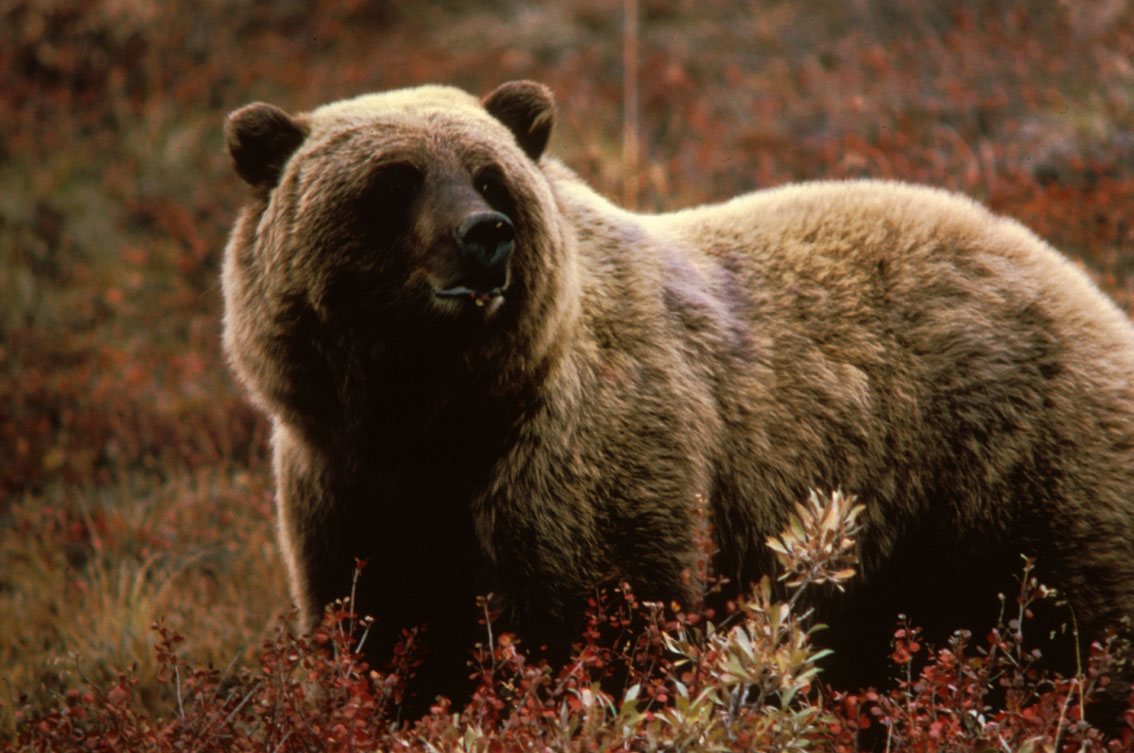
\includegraphics[width=\linewidth]{bear.jpg} % Figure image
	\caption{A majestic grizzly bear} % Figure caption
	\label{bear} % Label for referencing with \ref{bear}
\end{figure}

Aliquam elementum nulla at arcu finibus aliquet. Praesent congue ultrices nisl pretium posuere. Nunc vel nulla hendrerit, ultrices justo ut, ultrices sapien.  \todo{Maybe this can go to page 4} Duis ut arcu at nunc pellentesque consectetur. Vestibulum eget nisl porta, ultricies orci eget.

\begin{table}
	\caption{Example table}
	\centering
	\begin{tabular}{llr}
		\toprule
		\multicolumn{2}{c}{Name} \\
		\cmidrule(r){1-2}
		First Name & Last Name & Grade \\
		\midrule
		John & Doe & $7.5$ \\
		Richard & Miles & $5$ \\
		\bottomrule
	\end{tabular}
\end{table}

\section{Document Version control}

This section helps keeping track of all the changes done in the document. Here is where all the TODO notes go when they are resolved. And you would find something like this so it is not repeated again\\

\begin{table}
	\caption{Solved issues}
	\centering
	\begin{tabular}{lll}
		\toprule
		Date & Original & Solved \\
		\midrule
		2022.02.01 & Write something! & Abstract and Method added \\
		2022.02.02 & Definition of obesity is not included & Added definition according to the meeting we had on January \\
		\bottomrule
	\end{tabular}
\end{table}



%----------------------------------------------------------------------------------------
%	BIBLIOGRAPHY
%----------------------------------------------------------------------------------------

%\printbibliography[title={Bibliography}] % Print the bibliography, section title in curly brackets


\bibliography{bibliography} 
\bibliographystyle{ieeetr}


%----------------------------------------------------------------------------------------

%----------------------------------------------------------------------------------------
%	Supplementary material
%----------------------------------------------------------------------------------------

\onecolumn

\section{Suplementary material}

In this section, we present some useful extra information\\

\input{../../../../results/biomarkers/tables/LatexTable_SuplementaryAllBiomarkers.tex}	

\input{../../../../results/biomarkers/tables/LatexTable_SexDifferencesBiomakers.tex}	



\end{document}
